\documentclass[12pt]{article}
\usepackage{../../../format}
\lhead{A Level Physics - Turning Points}

%File specific preamble
\usetikzlibrary{scopes}

\begin{document}
\begin{center}
\underline{\huge Electrons}
\end{center}
\section{Discharge tube}
\begin{itemize}
\item As p.d. increased from 0V, initially no glow
\item p.d. increased further - suddenly glows can be seen and p.d. drops as the gas now conducts
\item Increasing p.d. further causes gas to glow brighter
\end{itemize}
When several kV is applied a narrow band "glow" causes gas to glow brighter
\subsection{Explanation of how it works}
\begin{itemize}
\item The high p.d. is sufficient to ionise the gas
\item The positive ions accelerate towards the cathode
\item The ions will hit the metal cathode with sufficient energy to release free electrons from the surface
\item The free electrons from the metal (low energy) can recombine with the gas ions-emitting photons and will be a continuous spectrum
\item The free electrons accelerate towards the anode. These free electrons will \textbf{inelastically} collide with gas atoms (and ions) causing bound electrons to be excited, then de-excited. This will produce a discrete spectrum which is seen in the positive column.
\end{itemize}
\section{Thermionic emission}
When a metal is heated the free electrons can gain enough energy to be released from the surface. This is called thermionic emission (similar to the photoelectric effect).\\
\\
In the presence of an electric field the thermionic electrons can be accelerated to form a narrow beam.\\
\\
When accelerated through a p.d. of \textbf{V} volts the electron gains \textbf{eV} in energy in the form of kinetic energy.
\newpage
\section{Determining the specific charge of an electron}
\subsection{Method 1}
1. Thermionic electrons are accelerated through a p.d. $V_a$ and gain kinetic energy:\\
$$eV_a=\frac{1}{2}mv^2 \quad \frac{e}{m}=\frac{\frac{1}{2}v^2}{\textrm{v}_a}$$
2. Electrons pass through an electric field (Field strength, E) and are deflected.\\
\\
3. A magnetic field (field strength, B) is applied at right angles to the E field until electron motion is again horizontal.
$$\textrm{At this point magnetic force=Electric force}$$
$$Bev=eE \quad v=\frac{E}{B}$$
$$\frac{e}{m}=\frac{1}{2\textrm{v}_a}\Bigg(\frac{E}{B}\Bigg)^2$$
\subsection{Method 2}
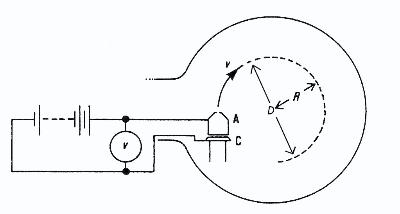
\includegraphics[width=10cm]{circluar_path.jpg}\\
Thermionic electrons are accelerated through a p.d. $V_a$\\
A magnetic field is applied perpendicular to the motion, causing the electrons to feel a force.\\
\\
$$\textrm{Magnetic force   F=Bev}$$
$$\textrm{This is the centripetal force,} \quad \frac{mv^2}{R}$$
$$\frac{e}{m}=\frac{v}{BR} \quad \quad v=\frac{e}{m}BR$$
$$\textrm{From accelerating p.d.}\quad eV_a=\frac{1}{2}mv^2$$
$$\frac{e}{m}=\frac{2V_a}{(BR)^2}$$
\newpage
\section{Milikan's experiment}
\begin{figure}[h]
    \centering
    \begin{minipage}{0.45\textwidth}
        \centering
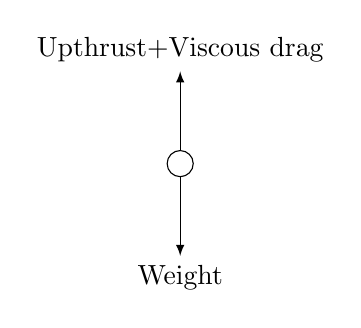
\begin{tikzpicture}[
    force/.style={>=latex,draw=black,fill=black},
    m/.style={circle,draw=black,fill=white,radius=0.3cm,thin},
]
    \node[m] (m) {};
    {[force,->]
        \draw (m.north) -- ++(0,1) node[above] {Upthrust+Viscous drag};
        \draw (m.south) -- ++(0,-1) node[below] {Weight};
    }
\end{tikzpicture}
        \caption{No electric field}
    \end{minipage}\hfill
    \begin{minipage}{0.45\textwidth}
        \centering
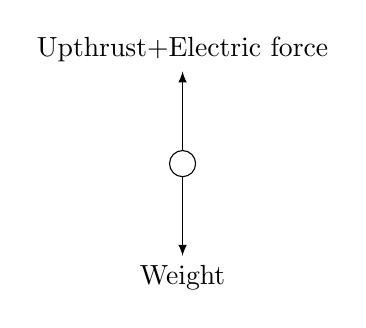
\begin{tikzpicture}[
    force/.style={>=latex,draw=black,fill=black},
    m/.style={circle,draw=black,fill=white,radius=0.3cm,thin},
]
    \node[m] (m) {};
    {[force,->]
        \draw (m.north) -- ++(0,1) node[above] {Upthrust+Electric force};
        \draw (m.south) -- ++(0,-1) node[below] {Weight};
    }
\end{tikzpicture}    
        \caption{Electric field}
    \end{minipage}
\end{figure}
\subsection{With electric field}
$$\textrm{Electric field}=\frac{QV}{d}$$
$$\textrm{Weight}=mg$$
$$\frac{QV}{d}=mg$$
\subsection{Without electric field}
$$F_D=6\pi r\eta v$$
$$\textrm{Weight}=mg$$
\begin{center}
Mass=Density$\times$Volume
$$\textrm{Mass}=\frac{4}{3}\pi r^3\rho$$
$$6\pi r\eta v=\frac{4}{3}\pi r^3\rho g$$
$$r^2=\frac{9\eta v}{2\rho g}$$
\end{center}
\subsection{Significance of results}
These results were significant because it introduced the idea of quantisation of charge
\newpage
\begin{center}
\underline{\huge Questions from past papers}
\end{center}
\section{Milikan's experiment}
\textit{Why does an oil droplet reach a constant speed when the plate voltage is switched off in Milikan's experiment}
\begin{center}
Weight pulls droplet down, reaches terminal velocity
\end{center}
$ $\\
\textit{Derive $r^2=\frac{9\eta v}{2\rho g}$}
$$F_D=6\pi r\eta v$$
$$\textrm{Weight}=mg$$
\begin{center}
Mass=Density$\times$Volume
$$\textrm{Mass}=\frac{4}{3}\pi r^3\rho$$
$$6\pi r\eta v=\frac{4}{3}\pi r^3\rho g$$
$$r^2=\frac{9\eta v}{2\rho g}$$
\end{center}
$ $\\
\textit{Determine the mass or radius of a droplet in Milikan's experiment}\\
$$\textrm{Speed}=\frac{\textrm{Distance}}{\textrm{Time}}$$
$$r=\sqrt{\frac{9\eta v}{2\rho g}}$$
$$m=\frac{4}{3}\pi r^3\rho$$
$ $\\
\textit{Charge from mass}
$$Q=\frac{mgd}{V}$$
$ $\\
\textit{Determine the sign of the charge carried by a stationary droplet in Milikan's experiment}
\begin{center}
Opposite to the charge of the top plate to ensure forces are balanced
\end{center}
$ $\\
\textit{Comment on the significance of a charge calculated in Milikan's experiment}
\begin{center}
It will be a multiple of the charge of an electron
\end{center}
\section{Electron Guns}
\textit{Speed of electrons from the voltage they are accelerated through a Voltage}\\
$$\frac{1}{2}mv^2=eV$$
$$v=\sqrt{\frac{eV}{\frac{1}{2}m}}$$
$ $\\
\textit{Why are there two power supplies in an electron gun?}
\begin{center}
One to cause thermionic emission, one to accelerate the electrons
\end{center}
\section{Electrons in magnetic fields}
\textit{Does the speed of an electron change in a magnetic field}
\begin{center}
No as force is perpendicular to velocity, meaning no work is done
\end{center}
$ $\\
\textit{Specific charge from radius of curvature, magnetic flux density and accelerating voltage}
$$\frac{1}{2}mv^2=eV$$
$$\frac{mv^2}{r}=BeV$$
$$\frac{e}{m}=\frac{2V}{B^2r^2}$$
$ $\\
\textit{What is the velocity of an electron when magnetic and electric fields are equal}
$$EQ=BQv$$
$$v=\frac{E}{B}$$
$ $\\
\textit{Velocity of electrons in a magnetic field}
$$\frac{mv^2}{r}=Bev$$
$$v=\frac{Ber}{m}$$
$ $\\
\textit{Why do electrons undergo circular motion in a magnetic field}
\begin{center}
Force perpendicular to motion, does not change speed, causes direction of motion to change
\end{center}
$ $\\
\section{Electrons in electric fields}
\textit{Draw the path of an electron beam in an electric field}
\begin{center}
Curves up while between plates, straight line continuing up after leaving plates
\end{center}
$ $\\
\textit{Specific charge of an electron from curving in an electric field}
$$ma=\frac{eV}{d}$$
\begin{center}
Calculate acceleration using SUVAT
\end{center}
$$\frac{ad}{V}=\frac{e}{m}$$
$ $\\
\textit{Specific charge from electric field strength}
$$EQ=mg$$
$$\frac{Q}{m}=\frac{g}{E}$$
$ $\\
\textit{Why does an electron beam in an electric field curve at an increasing angle to the horizontal}
\begin{center}
The electrons feel a constant force, meaning they have constant vertical acceleration, causing the vertical component of the velocity to increase, while the horizontal component is constant, causing an increasing angle.
\end{center}
\section{Thermionic emission}
\textit{Explain thermionic emission}
\begin{center}
The current heats the wire, meaning the electrons in the filament gain sufficient k.e. to leave the filament
\end{center}
$ $\\
\textit{Why must the filament be in an evacuated tube for thermionic emission}
\begin{center}
So that there are no collisions
\end{center}
$ $\\
\textit{Why is thermionic emission negligible when the filament current is too low}
\begin{center}
If the current is too low there is little heating effect, meaning that the electrons don't gain enough kinetic energy to be released
\end{center}
\section{Discharge Tubes}
\textit{Why is light emitted in a Crooke's tube}
\begin{center}
Electrons present, collide with atoms, excitation occurs, emit photon as they return to the ground state
\end{center}
$ $\\
\textit{Why can a glow not be seen until the pressure is low enough in a Discharge tube}
\begin{center}
The electrons can't gain enough kinetic energy as there are too many molecules present
\end{center}
$ $\\
\end{document}